\chapter{Results}
\label{chap:results}

This chapter presents the main results from the implemented \gls{SafeVision} system. The evaluation covers both pre-trained models integrated into the \gls{anonymization} pipeline and custom-trained models developed during the project. In addition, the chapter reports results from the video processing extension, including qualitative redaction examples, manual tracking accuracy, prediction-based frame coverage, and processing performance.

%------------------------11.1-------------------------

\section{Pre-Trained Model Results}

This chapter presents the results obtained using pre-trained models integrated into the \gls{anonymization} pipeline. The models were used without additional fine-tuning and evaluated directly within the full system. To provide context for the observed performance, benchmark results from the original implementations are included alongside qualitative and system-level observations.

\methodheading{Face Detection}

Face detection was performed using the pre-trained RetinaFace model through the PyTorch implementation provided by \texttt{biubug6/Pytorch\_Retinaface} \cite{biubug6_retinaface}.  Table~\ref{tab:retinaface_widerface} summarizes the reported validation performance on the WIDER FACE dataset using single-scale evaluation. The implementation provides results for both \texttt{ResNet50} and \texttt{MobileNet0.25} backbones. The \texttt{ResNet50} backbone achieves the strongest reported performance, with 94.82\%, 93.84\%, and 89.60\% on the easy, medium, and hard subsets, respectively, while the lightweight \texttt{MobileNet0.25} configuration achieves 88.67\%, 87.09\%, and 80.99\%.

\begin{table}[H]
\centering
\begin{tabular}{lccc}
\toprule
Backbone / Style & Easy & Medium & Hard \\
\midrule
ResNet50 (PyTorch, same parameters as MxNet) & 94.82\% & 93.84\% & 89.60\% \\
MobileNet0.25 (PyTorch, same parameters as MxNet) & 88.67\% & 87.09\% & 80.99\% \\
\bottomrule
\end{tabular}
\caption{Reported WIDER FACE validation performance of the RetinaFace PyTorch implementation using single-scale evaluation \cite{biubug6_retinaface}.}
\label{tab:retinaface_widerface}
\end{table}

These benchmark results provide context for the observed system performance, where RetinaFace produced stable and consistent face detections across a wide range of input images. In practice, the model was able to accurately localize faces under varying lighting conditions and moderate occlusions, and it maintained high detection confidence for most visible faces.

The precision--recall curves reported for the WIDER FACE validation set are shown in Figure~\ref{fig:retinaface_widerface_combined}. The curves illustrate the expected decrease in performance as the evaluation setting becomes more challenging. This trend was also reflected in the system, where detection performance was slightly reduced for small or heavily occluded faces, while remaining strong for clearly visible faces.

The precision--recall curves reported for the WIDER FACE validation set are shown in Figure~\ref{fig:retinaface_widerface_combined}. The figure is included as benchmark context and shows RetinaFace compared with other face detection methods on the easy, medium, and hard subsets of WIDER FACE. It does not distinguish between the \texttt{ResNet50} and \texttt{MobileNet0.25} backbones used in the PyTorch implementation; these backbone-specific results are instead reported in Table~\ref{tab:retinaface_widerface}. Overall, the curves show that RetinaFace performs competitively on WIDER FACE, while performance decreases as the evaluation subset becomes more challenging.

\begin{figure}[H]
\centering
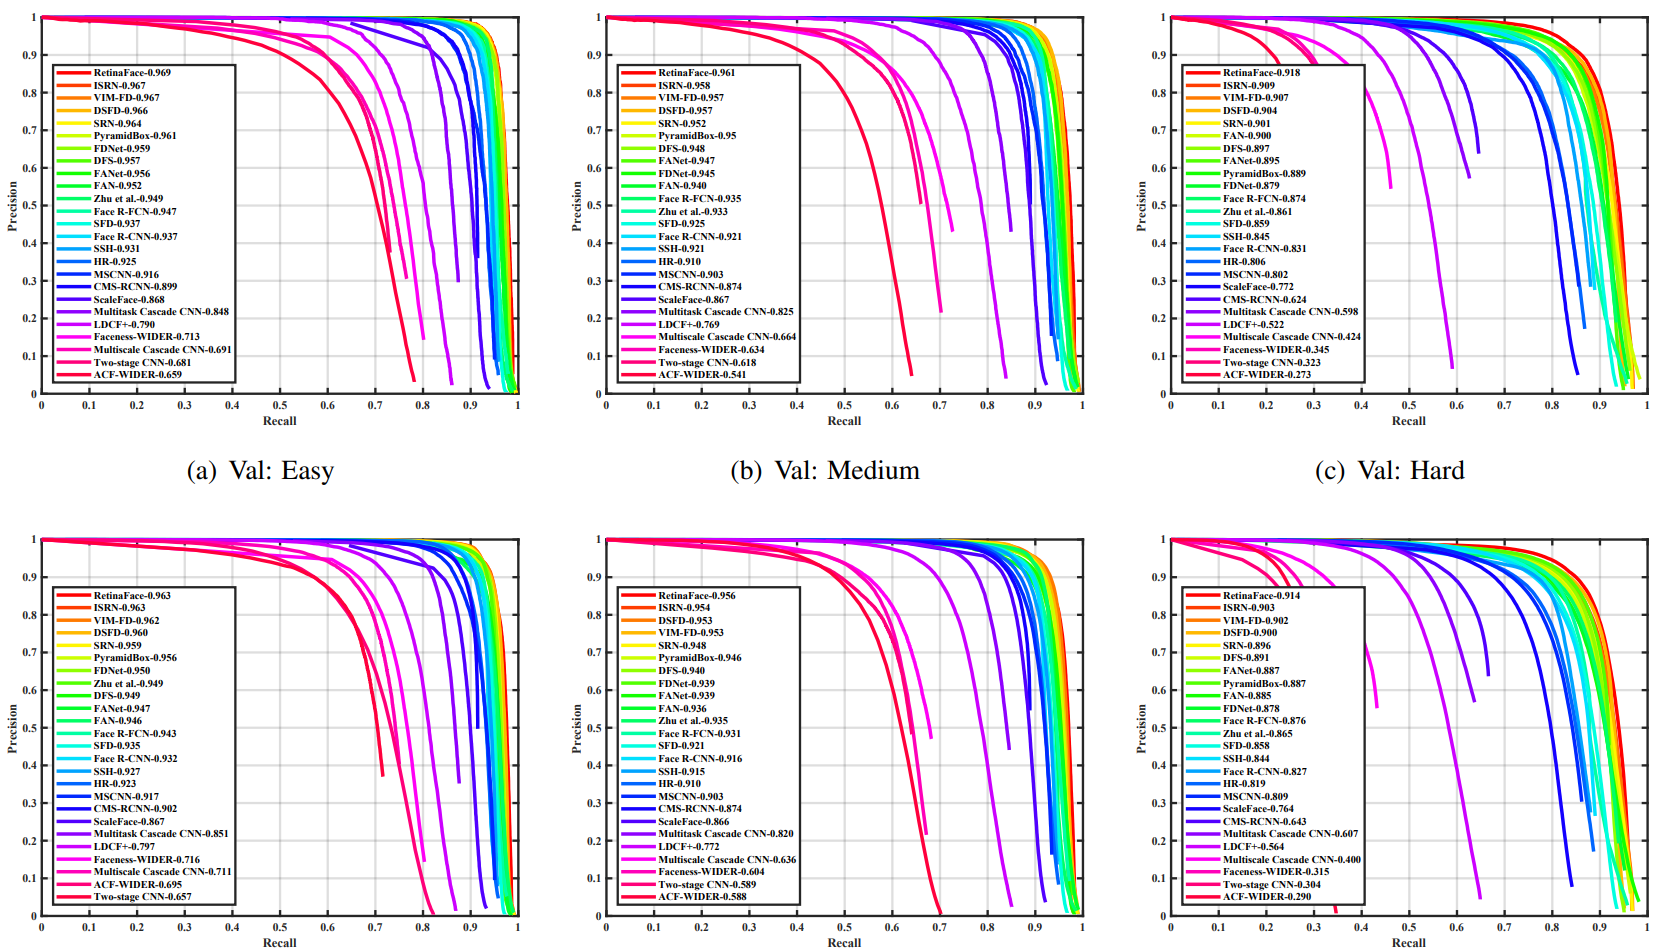
\includegraphics[width=\textwidth,height=0.50\textheight,keepaspectratio]{figures/images/chapter-11/retinaface/precision–recall-for-test-and-val-set.png}
\caption{Precision--recall curves for RetinaFace compared with other face detection methods on the WIDER FACE validation set, divided into easy, medium, and hard subsets \cite{deng2020retinaface}. Backbone-specific results for the PyTorch implementation are reported separately in Table~\ref{tab:retinaface_widerface}.}
\label{fig:retinaface_widerface_combined}
\end{figure}

In addition to WIDER FACE, the implementation also reports results on the FDDB benchmark, as shown in Table~\ref{tab:retinaface_fddb}. Both backbones achieve high performance, with \texttt{MobileNet0.25} reaching 98.64\% and \texttt{ResNet50} achieving 99.22\%.

\begin{table}[H]
\centering
\caption{Reported FDDB performance of the RetinaFace PyTorch implementation \cite{biubug6_retinaface}.}
\label{tab:retinaface_fddb}
\begin{tabular}{lc}
\toprule
Backbone & Performance \\
\midrule
MobileNet0.25 & 98.64\% \\
ResNet50 & 99.22\% \\
\bottomrule
\end{tabular}
\end{table}

The FDDB evaluation curves (Figure~\ref{fig:retinaface_fddb}) further indicate high true positive rates across a wide range of \gls{false positive} counts. This behavior was consistent with observations from the implemented system, where the model rarely produced false detections and maintained reliable localization.

\begin{figure}[H]
\centering
\makebox[\textwidth][c]{
    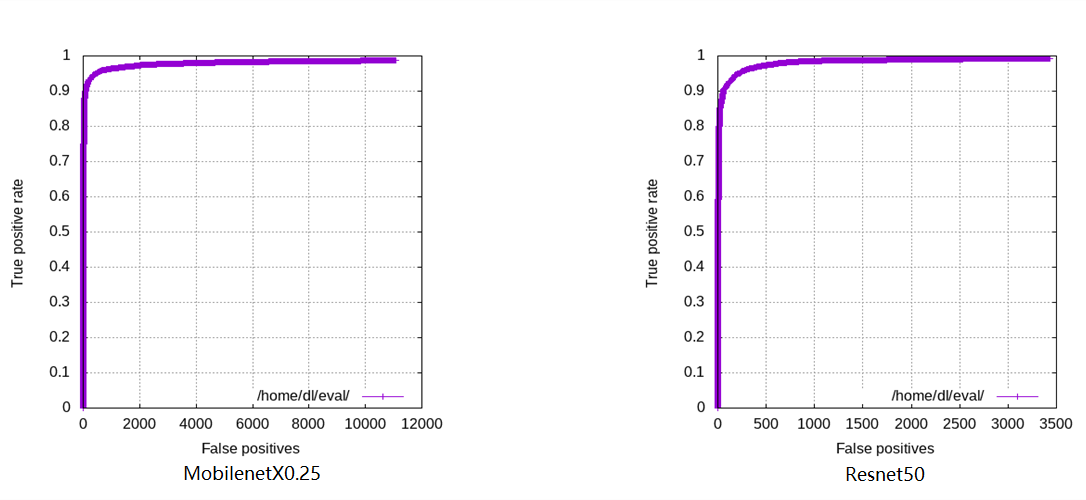
\includegraphics[width=1.2\textwidth]{figures/images/chapter-11/retinaface/fddb_curves.png}
}
\caption{FDDB evaluation curves reported for the RetinaFace implementation using the MobileNet0.25 and ResNet50 backbones \cite{biubug6_retinaface}.}
\label{fig:retinaface_fddb}
\end{figure}

The face detection component demonstrated reliable and consistent performance within the \gls{anonymization} pipeline. While minor performance degradation was observed for small or heavily occluded faces, the model provided sufficiently accurate detections for downstream \gls{anonymization}. This confirms that the pre-trained RetinaFace model is well-suited for real-time face detection in the proposed system.


\methodheading{Text Detection and Recognition}

Text detection and recognition were performed using pre-trained PaddleOCR models integrated into the \gls{anonymization} pipeline \cite{paddleocr_overview}. The system used the \texttt{PP-OCRv5\_mobile\_det} model for text detection and the \texttt{en\_PP-OCRv5\_mobile\_rec} model for text recognition, both executed on CPU. Table~\ref{tab:paddleocr_text_models} summarizes the reported benchmark results for the selected models. The detection model achieves an Hmean of 79.0, while the recognition model reports an average accuracy of 85.25. These values provide a reference for the observed system performance.

\begin{table}[!htbp]
\centering
\begin{tabular}{lcccc}
\toprule
Model & Task & Metric & CPU Time (ms) & Size (MB) \\
\midrule
PP-OCRv5\_mobile\_det & Detection & Hmean = 79.0 & 51.00 / 28.58 & 4.7 \\
en\_PP-OCRv5\_mobile\_rec & Recognition & Avg Accuracy = 85.25 & -- & 7.5 \\
\bottomrule
\end{tabular}
\caption{Official PaddleOCR benchmark results for the text detection and recognition models used in the system \cite{paddleocr_model_list_2x}.}
\label{tab:paddleocr_text_models}
\end{table}

In the implemented system, PaddleOCR produced accurate and consistent text localization across both document-like and natural scene images. The detection model generated tight \gls{bounding box}es around text regions, while the recognition model correctly transcribed most detected text, including multi-line and structured content.

Unlike the RetinaFace evaluation, detailed precision--recall curves were not available for the selected PaddleOCR configuration. The official documentation instead provides aggregate benchmark metrics, which limits direct comparison of detection behavior across varying thresholds. As a result, qualitative system-level examples are included to illustrate performance in practical scenarios. Figure~\ref{fig:text_detection_recognition_examples} presents examples of text detection and recognition results. In the document-like example, the model demonstrates high accuracy in detecting structured text, with precise localization and correct recognition of multiple lines. In the scene example, the model successfully identifies text under more challenging conditions, including varying backgrounds, perspective distortion, and uneven lighting.

\begin{figure}[H]
    \centering

    \begin{minipage}{\textwidth}
        \centering
        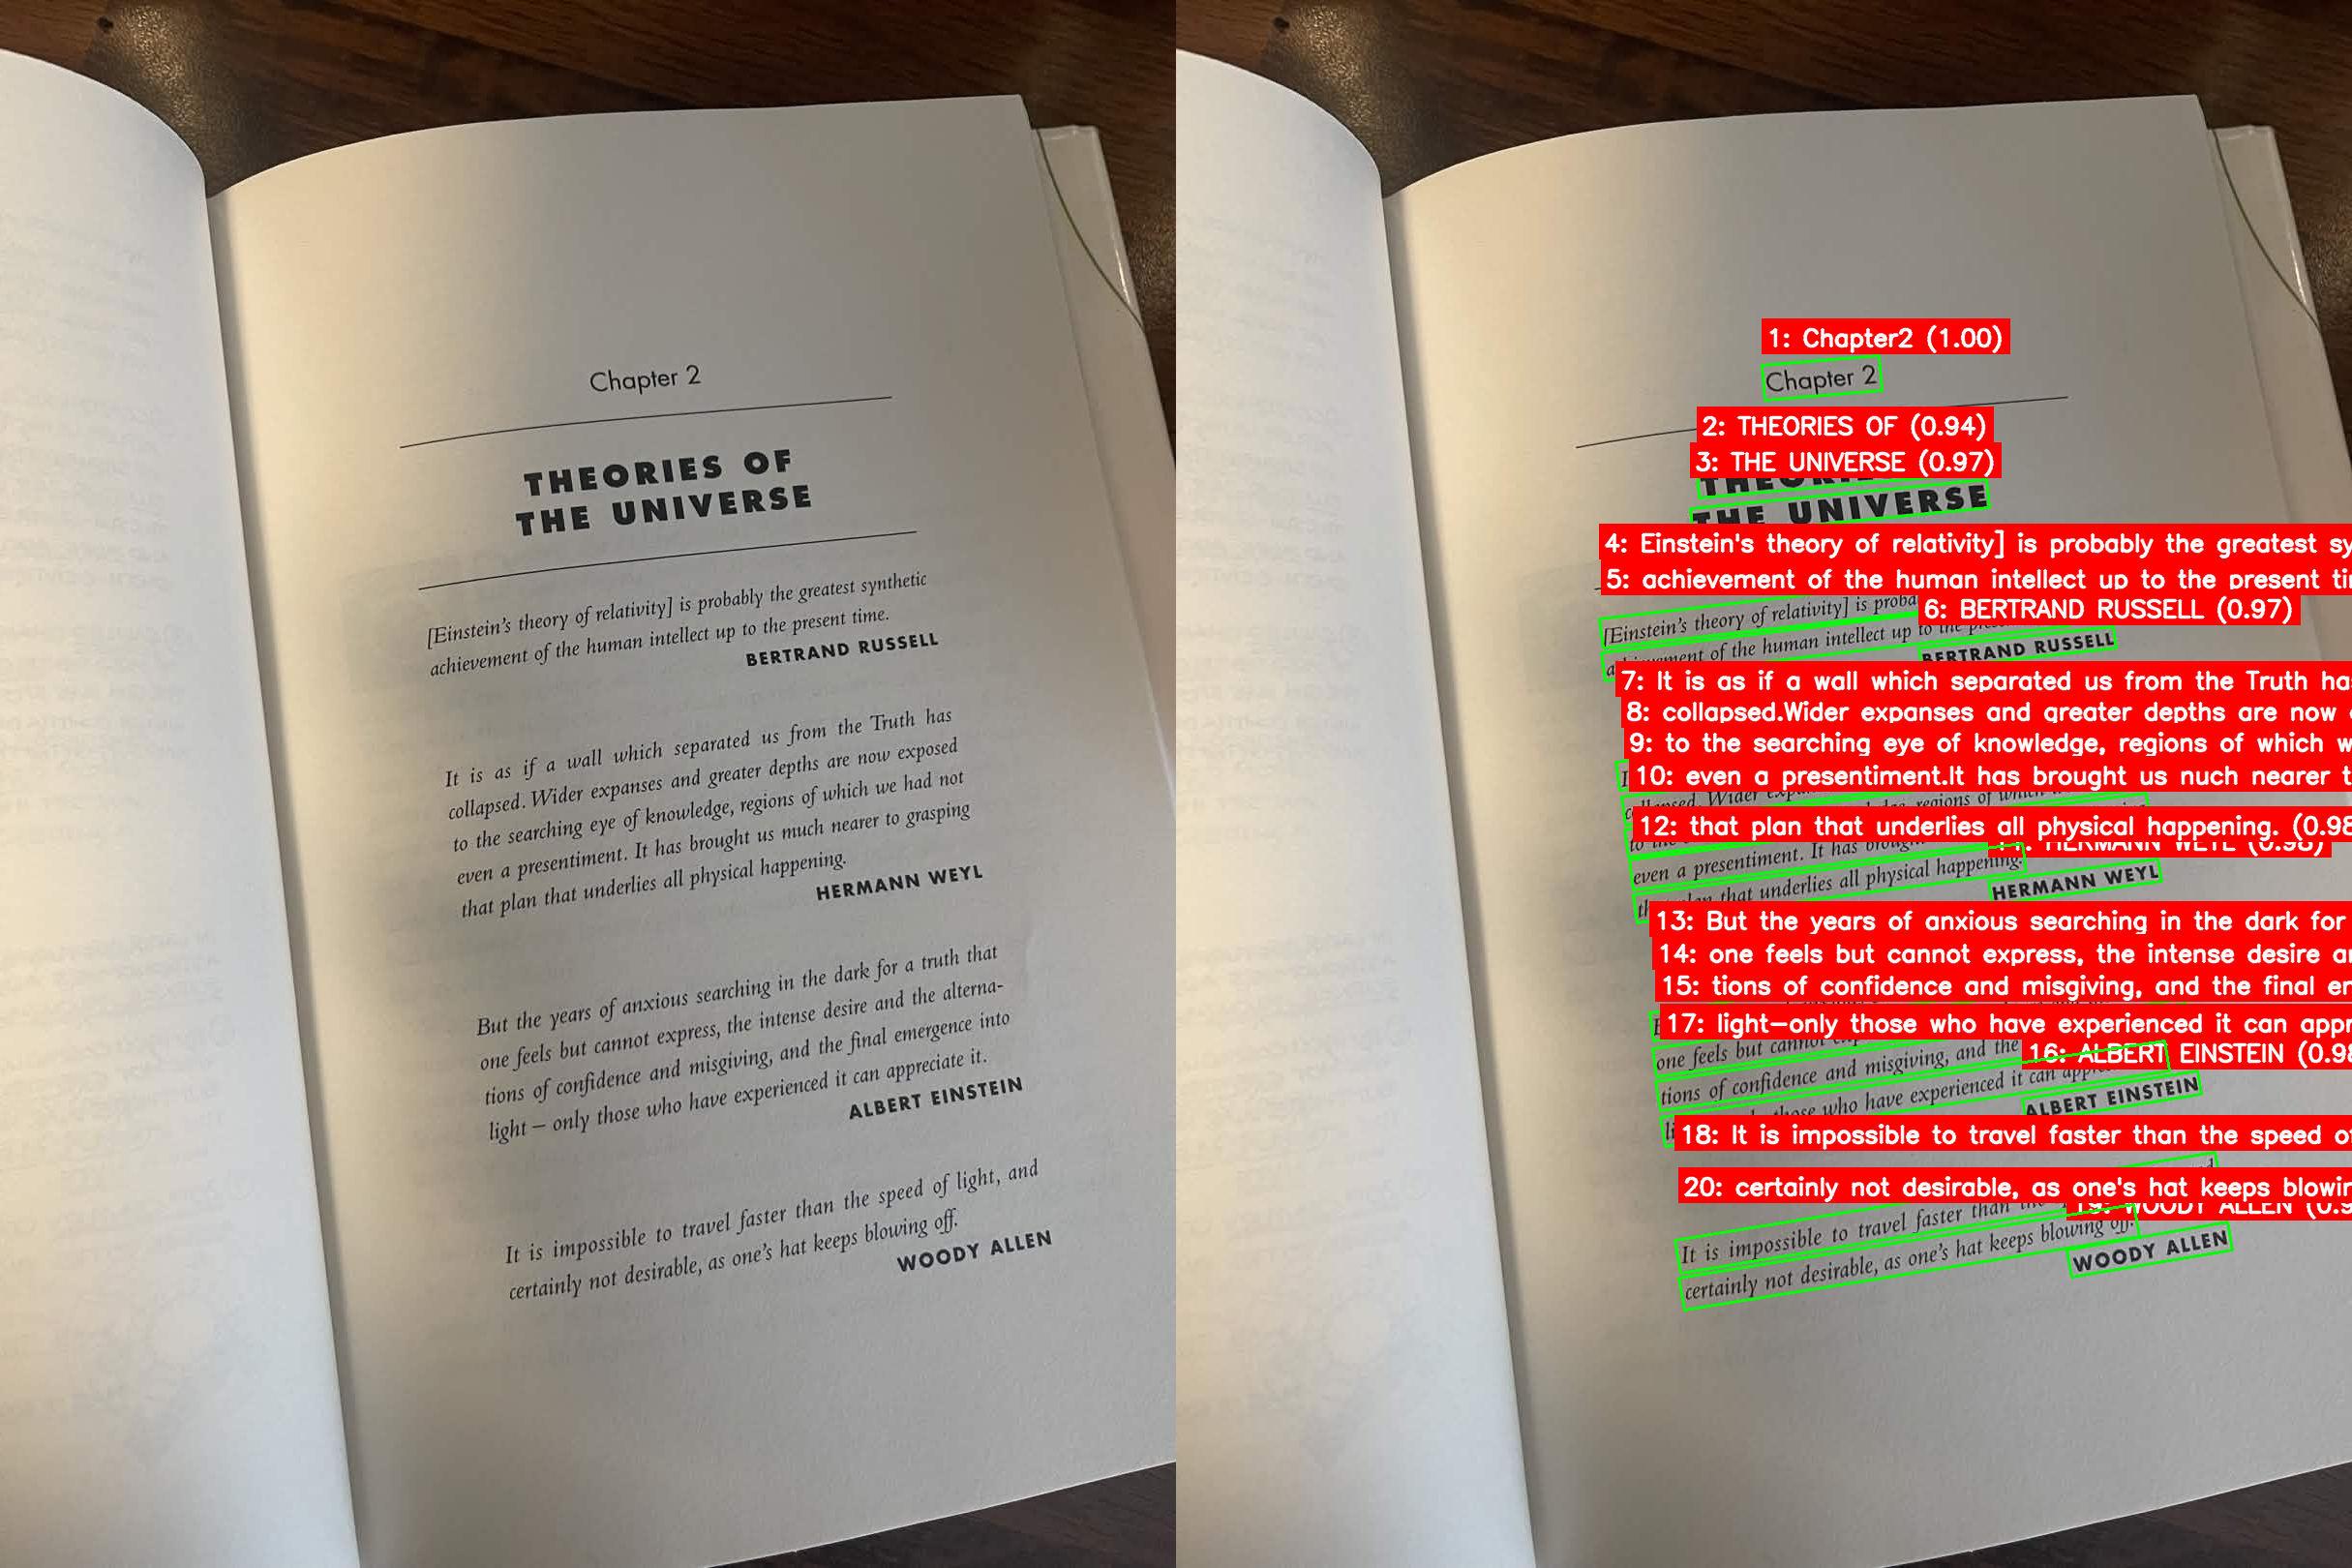
\includegraphics[width=1.0\textwidth]{figures/images/chapter-11/text-detection/IMG_7358_ocr_comparison.png}
        \par\vspace{2pt} \small (a) Example from a document-like image (Photo by author. Source: \textit{A Brief History of Time} \cite{hawking2017}).
    \end{minipage}

    \vspace{0.0cm}

    \begin{minipage}{\textwidth}
        \centering
        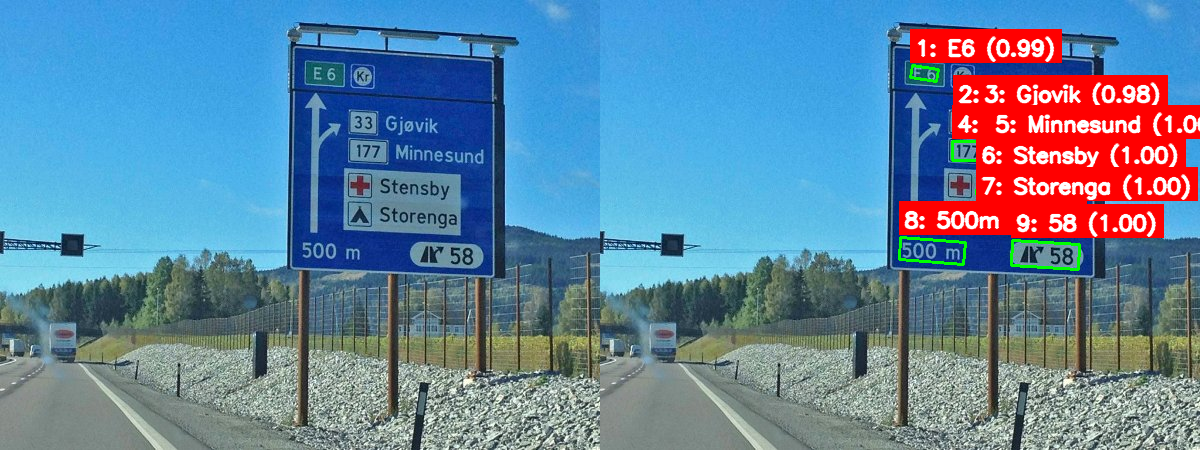
\includegraphics[width=1.0\textwidth]{figures/images/chapter-11/text-detection/gjovik_ocr_comparison.png}
        \par\vspace{2pt} \small (b) Example from a scene image (Image source: \cite{smaalenene2014}).
    \end{minipage}

    \caption{Representative text detection and recognition results produced by PaddleOCR in the integrated \gls{anonymization} pipeline.}
    \label{fig:text_detection_recognition_examples}
\end{figure}

While the overall performance was strong, some limitations were observed. Recognition accuracy decreased for small, low-resolution, or low-contrast text, particularly in complex scene images. Minor errors such as incorrect characters or missed spaces were occasionally present, although these did not significantly impact the \gls{anonymization} process. Despite these limitations, the models maintained stable performance across diverse input conditions and operated efficiently on CPU (Section~\ref{sec:performance_tests}), enabling responsive \gls{inference} within the pipeline. The PaddleOCR-based component provided sufficiently accurate text localization and recognition for reliable \gls{anonymization} in the proposed system.


\methodheading{General Object Detection}

General \gls{object detection} was performed using a pre-trained \gls{yolox-s} model integrated into the \gls{anonymization} pipeline \cite{yolox}. The same model architecture was also used for the custom-trained barcode and license plate detectors, resulting in consistent detection behavior across components.

To make the general object detector more suitable for \gls{SafeVision}, the original COCO output classes were reduced to a smaller set of privacy-relevant categories which contains 80 object classes. In this project, these classes are mapped to a smaller set of application-specific categories, including \texttt{PERSON}, \texttt{VEHICLE}, \texttt{ANIMAL}, \texttt{BAG}, \texttt{ELECTRONIC}, and \texttt{STREET\_OBJECT}. This mapping simplifies the detection output and allows the system allows the system to prioritize entities for \gls{anonymization}. Classes not relevant for the application are filtered out during postprocessing.

\gls{yolox} is a one-stage object detector designed for efficient and real-time \gls{inference} \cite{yolox}. The \gls{yolox-s} variant used in this project provides a good balance between detection accuracy and computational efficiency, making it suitable for deployment in practical applications. Reported benchmark results on the COCO dataset show that \gls{yolox} achieves competitive performance compared to other real-time detectors \cite{yolox}. As shown in Table~\ref{tab:yolox_benchmark}, the \gls{yolox-s} model achieves approximately 40.5 AP while maintaining real-time \gls{inference} speed.

\begin{table}[H]
\centering
\begin{tabular}{lcc}
\toprule
Model & AP (COCO) & Frames Per Second (\acrshort{fps}) \\
\midrule
\gls{yolox-s} & $\sim$40.5 & $\sim$60+ \acrshort{fps} \\
\bottomrule
\end{tabular}
\caption{Reported \gls{yolox} performance on the COCO dataset (\gls{yolox-s} variant) \cite{yolox}.}
\label{tab:yolox_benchmark}
\end{table}

Figure~\ref{fig:yolox_benchmark_tradeoff} illustrates the relationship between model complexity and detection performance for \gls{yolox} and comparable models. The \gls{yolox-s} variant achieves a strong balance between accuracy and efficiency, outperforming several lightweight alternatives while maintaining a relatively low number of parameters.

\begin{figure}[H]
\centering
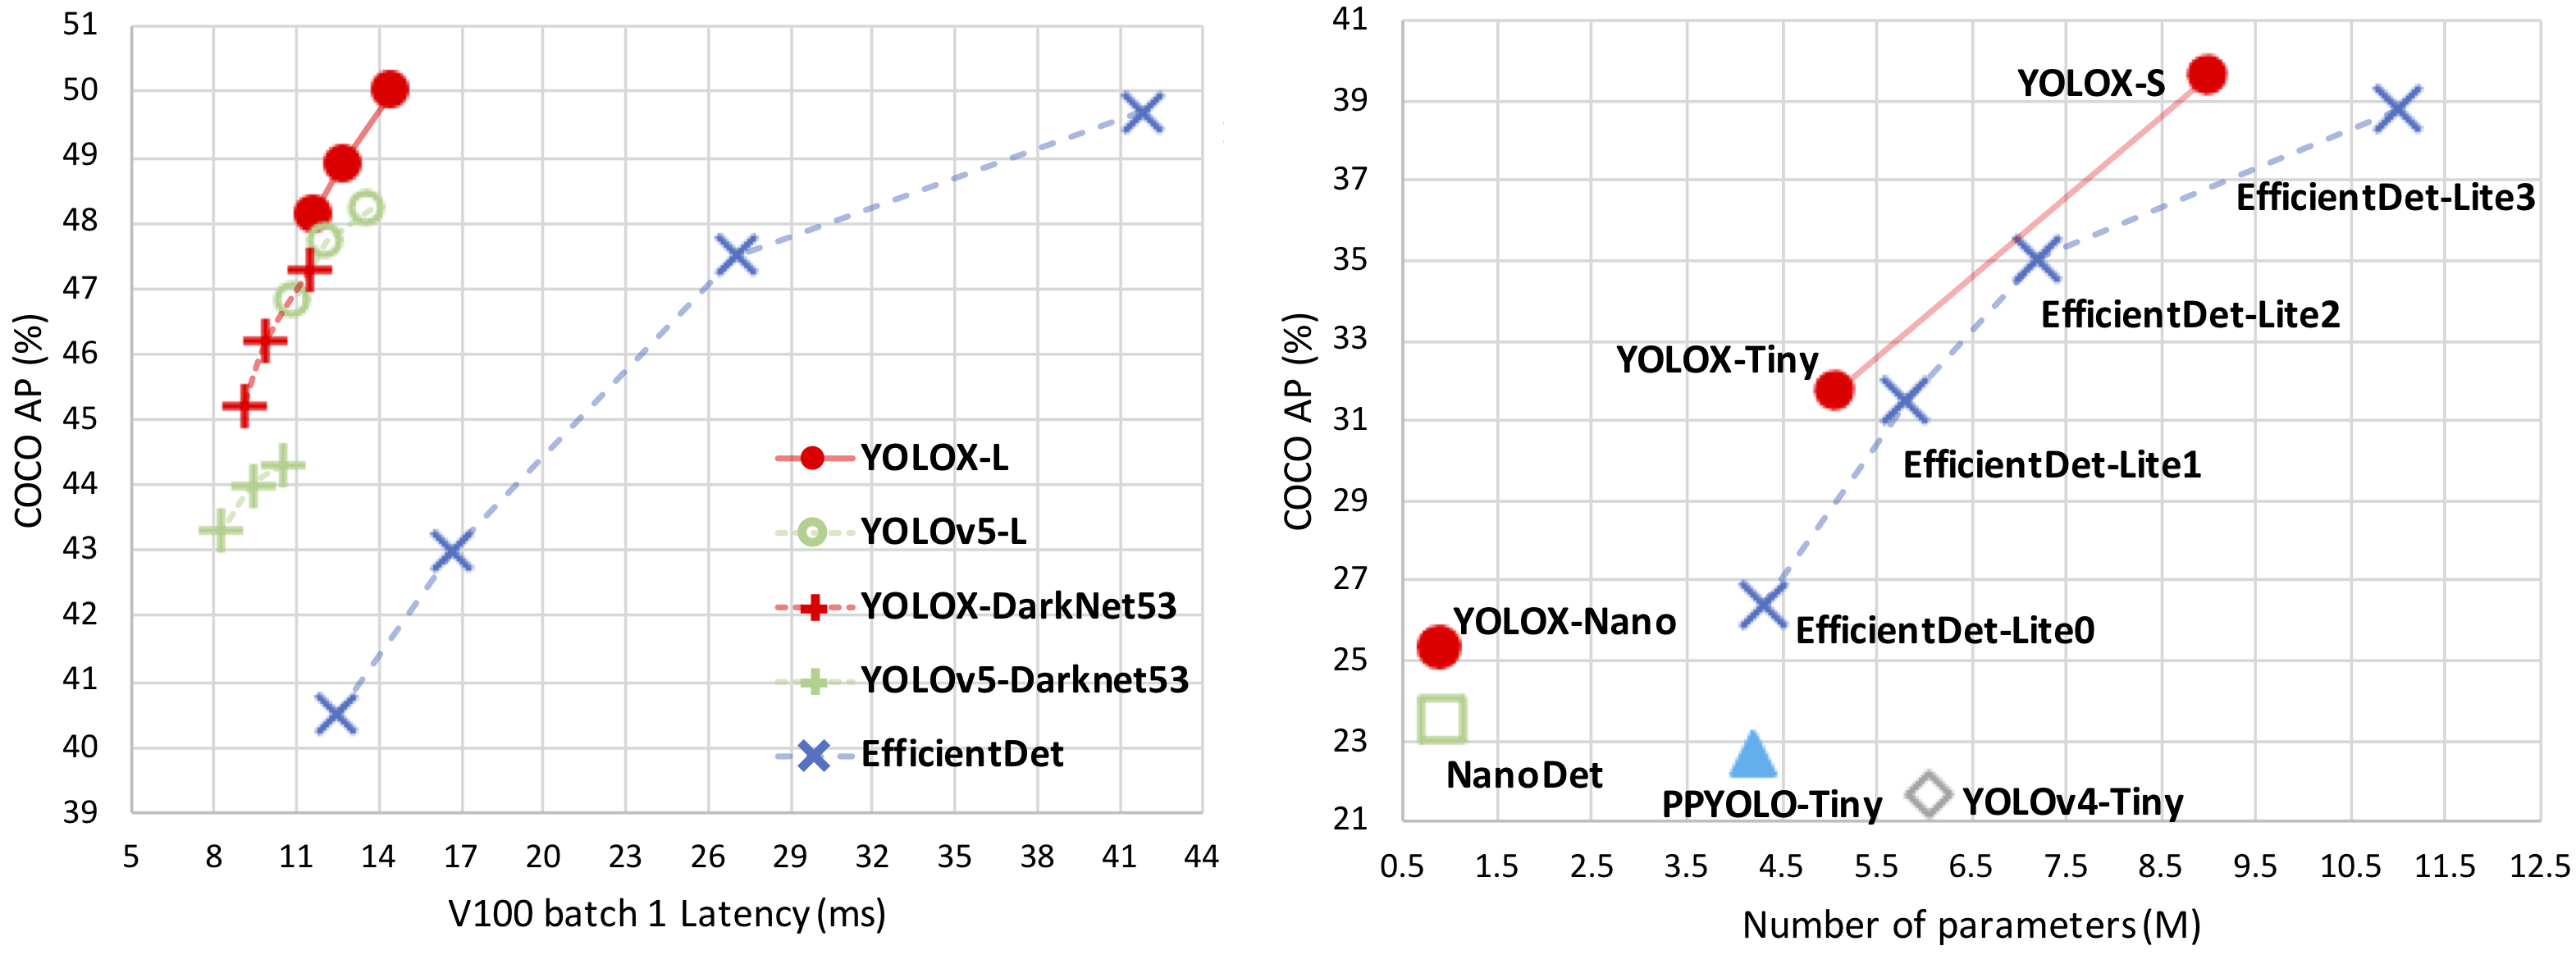
\includegraphics[width=1.1\textwidth]{figures/images/chapter-11/yolox/yolox_tradeoff.png}
\caption{Comparison of \gls{object detection} models showing the relationship between number of parameters and COCO AP. \gls{yolox-s} achieves a favorable balance between accuracy and model complexity \cite{yolox}.}
\label{fig:yolox_benchmark_tradeoff}
\end{figure}

Figure~\ref{fig:yolox_detection_example} shows an example of \gls{object detection} using the \gls{yolox} model in the implemented system. The model successfully detects multiple object types in the scene and assigns them to the corresponding application-specific categories.

\begin{figure}[H]
\centering
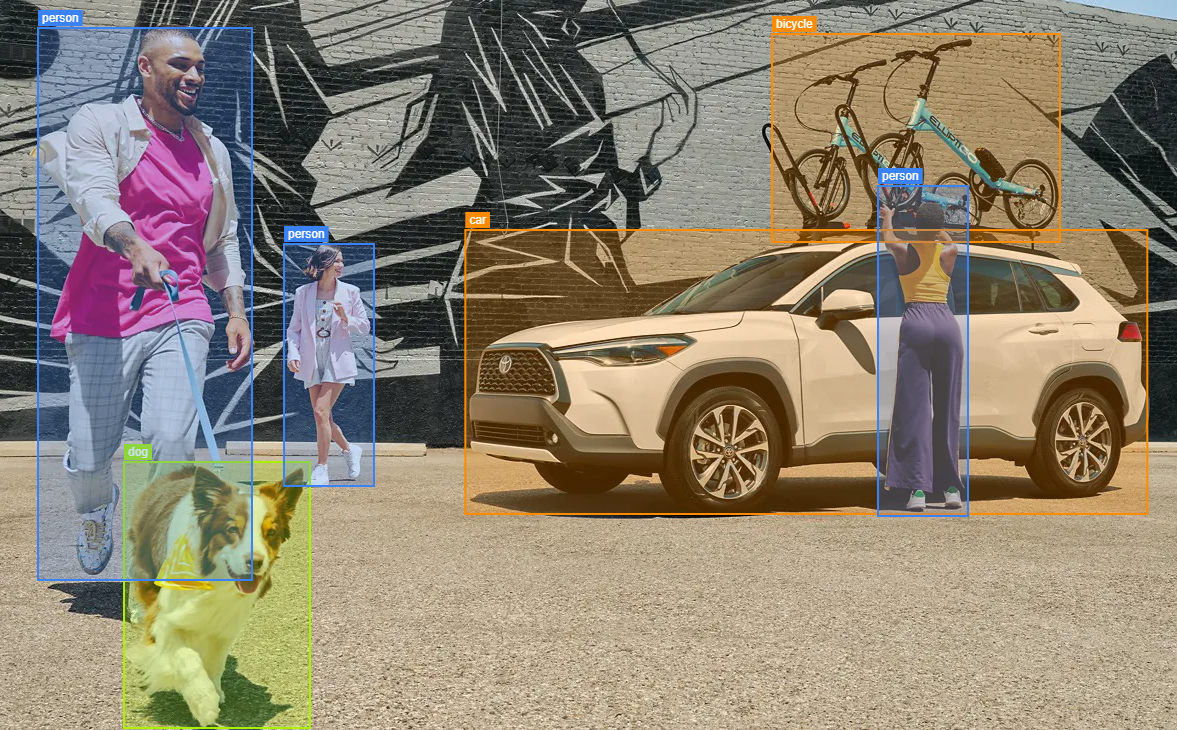
\includegraphics[width=1.1\textwidth]{figures/images/chapter-11/yolox/example.png}
\caption{Example of \gls{object detection} using YOLOX. The figure shows detected objects and their corresponding categories used in the \gls{anonymization} pipeline (Image source: \cite{foxdealer2024}).}
\label{fig:yolox_detection_example}
\end{figure}

YOLOX-based \gls{object detection} component provides reliable detection of general objects and complements the custom-trained models by covering a broader set of categories. This improves the robustness of the \gls{anonymization} system in real-world scenarios.

\methodheading{Image \Gls{segmentation}}

Image \gls{segmentation} was performed using the pre-trained \gls{mobilesam} model integrated into the \gls{anonymization} pipeline. Unlike \gls{object detection} models that produce \gls{bounding box}es, \gls{mobilesam} generates pixel-level \gls{segmentation} masks, enabling more precise \gls{anonymization} of detected objects.

In the implemented system, \gls{segmentation} was applied only within detected \gls{bounding box}es. This reduced unnecessary computation and ensured that \gls{segmentation} was limited to relevant regions, improving both efficiency and output quality. Figure~\ref{fig:segmentation_comparison} shows a comparison between \gls{bounding box} based \gls{anonymization} and \gls{segmentation} based \gls{anonymization}. The results demonstrate that \gls{mobilesam} produces masks that closely follow object boundaries, significantly reducing the inclusion of background regions. This was beneficial for irregularly shaped objects, where \gls{bounding box}es often covered large amounts of irrelevant area.

\begin{figure}[H]
\centering
\begin{subfigure}{0.32\textwidth}
\centering
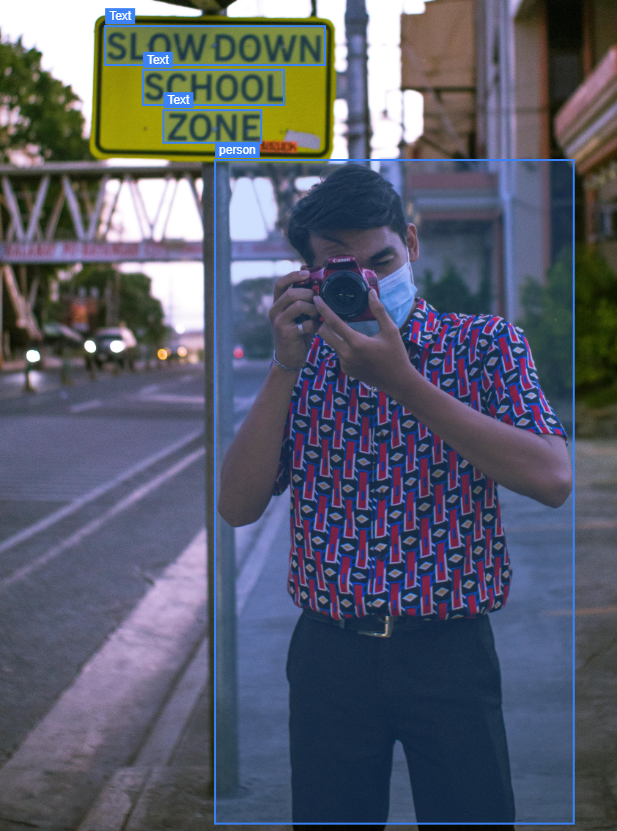
\includegraphics[width=\linewidth]{figures/images/chapter-11/segmentation/detection.png}
\caption{Detections filtered}
\end{subfigure}
\hfill
\begin{subfigure}{0.32\textwidth}
\centering
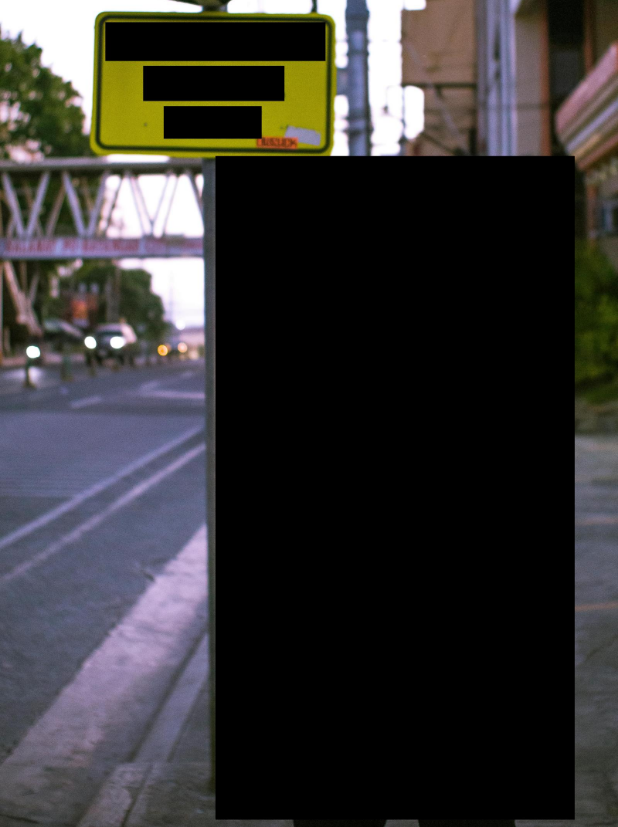
\includegraphics[width=\linewidth]{figures/images/chapter-11/segmentation/redaction-box.png}
\caption{Without \gls{segmentation}}
\end{subfigure}
\hfill
\begin{subfigure}{0.32\textwidth}
\centering
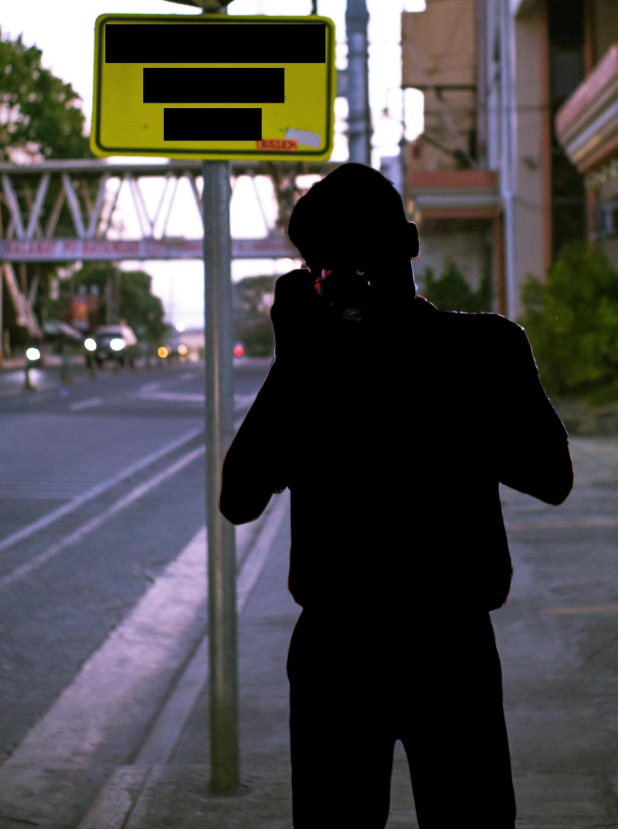
\includegraphics[width=\linewidth]{figures/images/chapter-11/segmentation/redaction-segmented.png}
\caption{With \gls{segmentation}}
\end{subfigure}
\caption{Comparison of \gls{anonymization} with and without \gls{segmentation}. (a) Detected region, (b) \gls{bounding box} based \gls{anonymization}, and (c) \gls{segmentation} based \gls{anonymization} using \gls{mobilesam}. Text regions are not segmented. (Image source from \cite{pavel2021})}
\label{fig:segmentation_comparison}
\end{figure}

In practice, \gls{mobilesam} produced stable and high-quality \gls{segmentation} masks across a range of object types. The masks were generally well-aligned with object boundaries, leading to more visually precise \gls{anonymization} compared to \gls{bounding box} based approaches. However, some limitations were observed. \Gls{segmentation} quality decreased for very small or low-resolution objects, and slight boundary inaccuracies were occasionally present in complex scenes with overlapping objects or weak contrast. Despite this, the \gls{segmentation} output remained sufficiently accurate for the intended \gls{anonymization} task.

Table~\ref{tab:mobilesam_comparison} summarizes benchmark results reported for \gls{mobilesam}. Compared to the original \acrshort{sam}, \gls{mobilesam} is significantly more efficient while maintaining similar \gls{segmentation} performance. These results are consistent with observations from the implemented system, where \gls{segmentation} added only a small computational overhead and remained suitable for near real-time processing. This made it well-suited for integration into the real-time \gls{anonymization} pipeline

\begin{table}[H]
\centering
\begin{tabular}{lcc}
\toprule
Metric & SAM & MobileSAM \\
\midrule
Model size & $\sim$632M params & $\sim$5.8M params \\
Speed & Baseline & 5--38$\times$ faster \\
\Gls{inference} time & $\sim$50--100 ms & $\sim$10 ms \\
m\acrshort{iou} & $\sim$0.76--0.78 & $\sim$0.74 \\
\bottomrule
\end{tabular}
\caption{Comparison between \acrshort{sam} and \gls{mobilesam} based on reported benchmark results \cite{mobilesam}.}
\label{tab:mobilesam_comparison}
\end{table}

%------------------------11.2-------------------------

\section{Custom-Trained Detection Models}
\label{sec:custom_trained_detection_models}

Two custom \gls{object detection} models were developed in this project: one for barcode detection and one for license plate detection. This section presents the final test-set results and the final models selected for use in the proposed system. Detailed training configurations, training curves, precision--recall curves, and confusion matrices are provided in Appendix~\ref{app:custom_model_evaluation}.

\methodheading{Barcode Detection Results}

\begin{figure}[H]
\centering
\begin{subfigure}{0.40\textwidth}
\centering
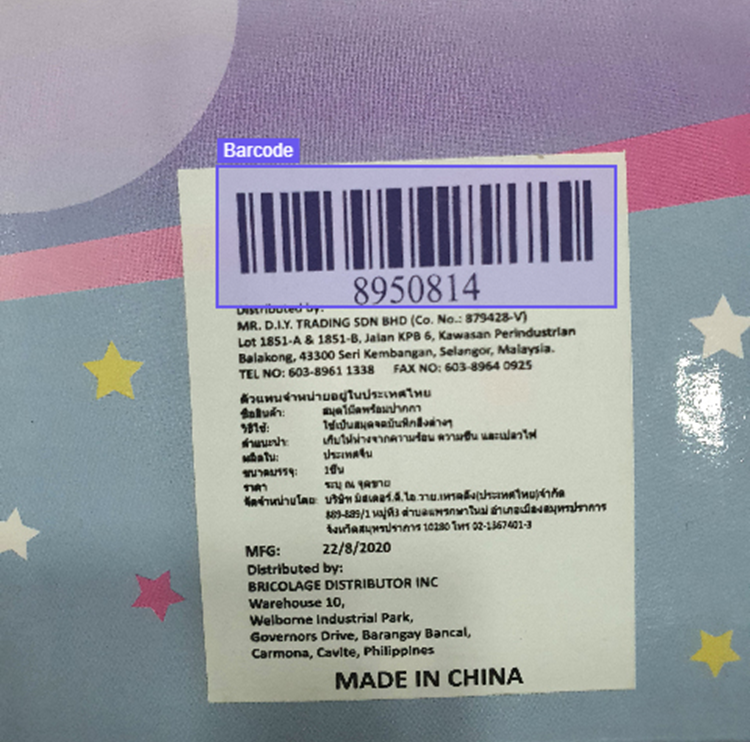
\includegraphics[width=\linewidth]{figures/images/chapter-11/qr-bar/example01.png}
\end{subfigure}
\hfill
\begin{subfigure}{0.40\textwidth}
\centering
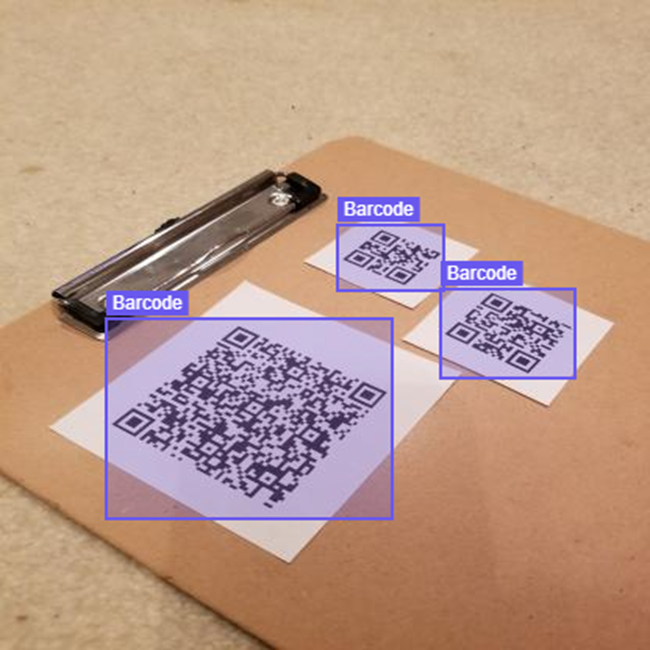
\includegraphics[width=\linewidth]{figures/images/chapter-11/qr-bar/example02.png}
\end{subfigure}
\caption{Examples of barcode and QR-code detection. Images from the test set, sources \cite{benchmark_barcode_kaggle,barcode_qr_kaggle}.}
\label{fig:qr_bar_examples}
\end{figure}

The final barcode detection model was evaluated on an unseen test set. Since the model achieved strong performance across all evaluation metrics, no further barcode model iterations were considered necessary.

\begin{table}[H]
\centering
\caption{Final barcode detection performance at confidence threshold $0.3$.}
\begin{tabular}{lcccccc}
\toprule
Model & TP & FP & FN & Precision & Recall & F1 Score \\
\midrule
Final barcode model & 1699 & 53 & 7 & 96.97\% & 99.59\% & 0.983 \\
\bottomrule
\end{tabular}
\label{tab:barcode_results}
\end{table}

As shown in Table~\ref{tab:barcode_results}, the barcode model achieved high precision and recall. The model missed 7 barcodes on the test set, indicating that it is reliable for detecting barcode and QR-code objects in the proposed system.

\methodheading{License Plate Detection Results}

\begin{figure}[H]
\centering
\begin{subfigure}{0.48\textwidth}
\centering
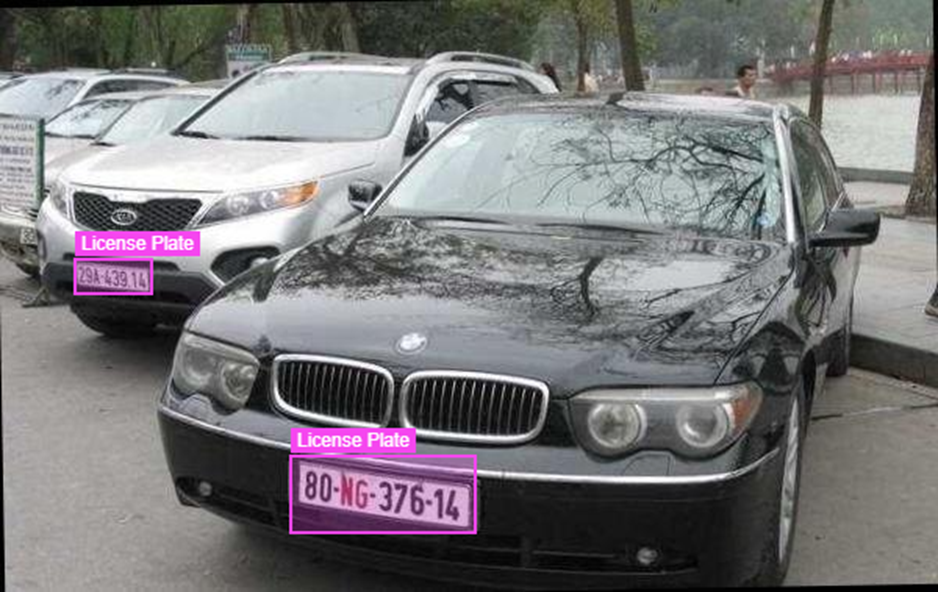
\includegraphics[width=\linewidth]{figures/images/chapter-11/licenseplate/example01.png}
\end{subfigure}
\hfill
\begin{subfigure}{0.48\textwidth}
\centering
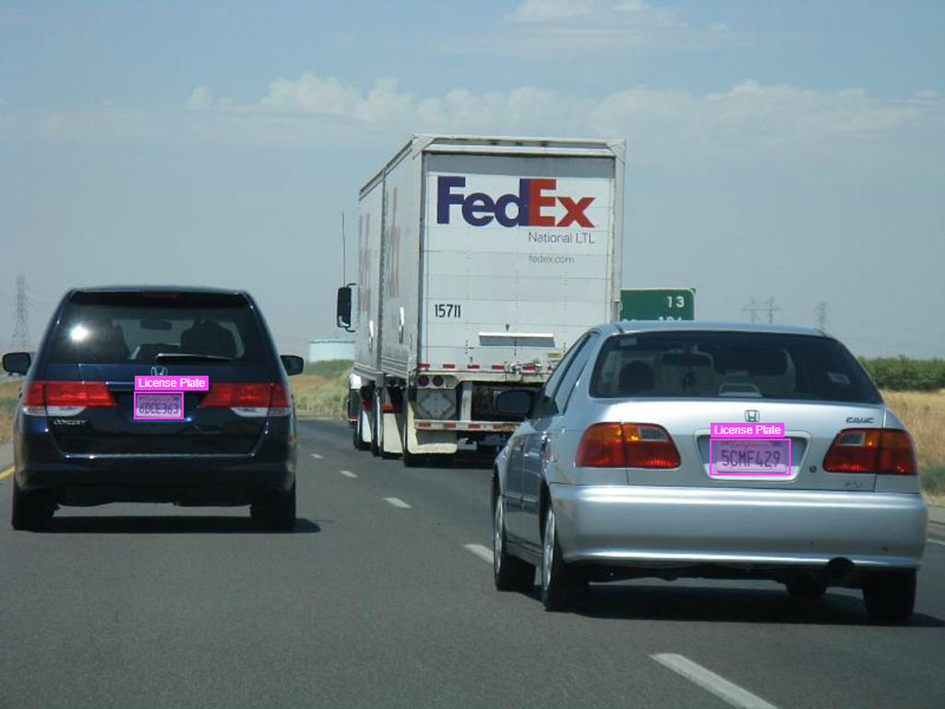
\includegraphics[width=\linewidth]{figures/images/chapter-11/licenseplate/example02.png}
\end{subfigure}
\caption{Examples of license plate detection. Images from the test set, sources \cite{lp_dataset_1,lp_dataset_2}.}
\label{fig:licenseplate_examples}
\end{figure}

For license plate detection, two configurations were evaluated to investigate the effect of increased input resolution on detection performance. Model v1 achieved slightly higher precision, while model v0 achieved higher recall and a higher F1-score.

\begin{table}[H]
\centering
\caption{License plate detection performance at confidence threshold $0.3$.}
\begin{tabular}{lccccccc}
\toprule
Model & Input Size & TP & FP & FN & Precision & Recall & F1 Score \\
\midrule
v0 & $640\times640$ & 1946 & 98 & 111 & 95.21\% & 94.60\% & \textbf{0.949} \\
v1 & $960\times960$ & 1964 & 80 & 186 & \textbf{96.09\%} & 91.35\% & 0.937 \\
\bottomrule
\end{tabular}
\label{tab:license_plate_results}
\end{table}

As shown in Table~\ref{tab:license_plate_results}, v1 produced fewer \gls{false positive}s and therefore achieved slightly higher precision. However, v0 missed fewer license plates and achieved the highest recall and F1-score. Since the proposed system benefits from detecting as many license plates as possible while still maintaining high precision, the v0 configuration was selected as the final license plate detection model. Further details for both license plate models are provided in
Appendix~\ref{app:license_plate_results}.

\methodheading{Named Entity Recognition Results}

\label{sec:ner_results}
The final NER model was evaluated on a held-out test split constructed from the merged training pipeline. The model achieved high aggregate scores on this test split.

\begin{table}[H]
\centering
\caption{Final NER model performance on the constructed held-out test split.}
\begin{tabular}{lcccc}
\toprule
Model & Loss & Precision & Recall & F1 Score \\
\midrule
Final NER model & 0.0061 & 99.73\% & 99.78\% & 0.9975 \\
\bottomrule
\end{tabular}
\label{tab:ner_results_main}
\end{table}

Although the NER model achieved near-perfect results on the constructed held-out test split, these results were not considered fully representative of practical system performance. Since the test split was derived from the same synthetic and
converted-data pipeline used during training, it remained relatively close to the training distribution.

\begin{table}[H]
\centering
\caption{Overall NER performance on the harder \acrshort{ocr} oriented test set.}
\begin{tabular}{lccc}
\toprule
Evaluation set & Precision & Recall & F1 Score \\
\midrule
Hard test set & 91.32\% & 96.13\% & 0.9366 \\
\bottomrule
\end{tabular}
\label{tab:ner_results_hard}
\end{table}

Additional evaluation on a separate harder \acrshort{ocr} oriented test set was performed. As shown in Table~\ref{tab:ner_results_hard}, the NER model achieved lower performance on the harder \acrshort{ocr} oriented test set than on the constructed held out split. This indicates that the near perfect results on the merged test split overestimated the model’s practical robustness, particularly in noisier and more semantically ambiguous \acrshort{ocr} scenarios.


\begin{figure}[H]
\centering
\begin{subfigure}{0.60\textwidth}
\centering
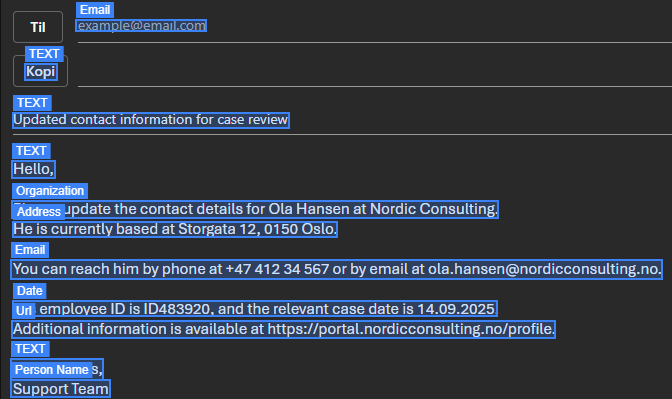
\includegraphics[width=\linewidth]{figures/images/chapter-11/ner/email.png}
\caption{Self-produced illustrative email example.}
\end{subfigure}
\hfill
\begin{subfigure}{0.60\textwidth}
\centering
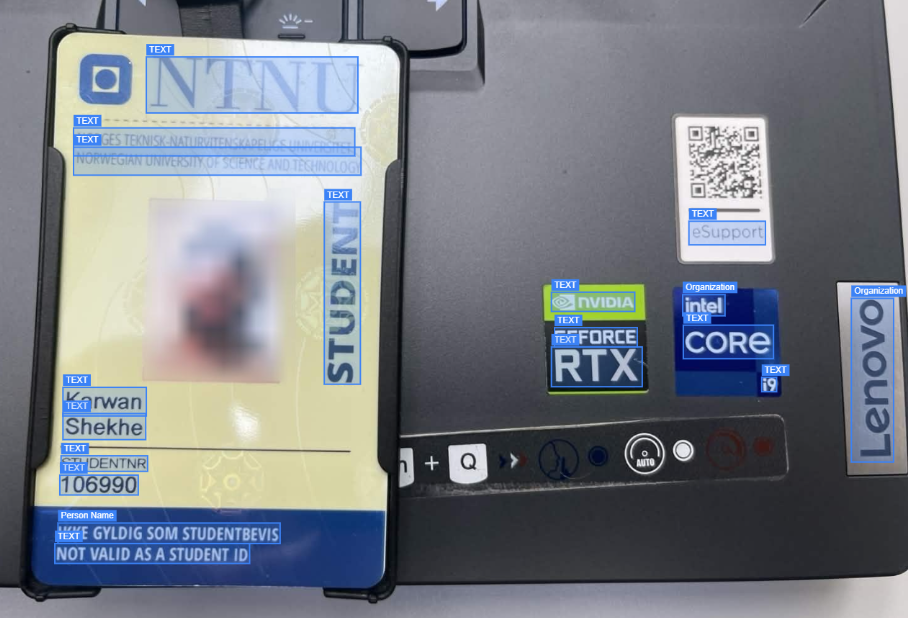
\includegraphics[width=\linewidth]{figures/images/chapter-11/ner/student-id.png}
\caption{Real-world student ID example.}
\end{subfigure}
\caption{Examples of \acrshort{ocr} based text categorization. Photos by the authors.}
\label{fig:ner_real_vs_controlled}
\end{figure}

Even though the evaluation on the constructed test split shows a high score, Figure~\ref{fig:ner_real_vs_controlled} indicates that the NER-based text categorization is not yet well suited for real-life document scenarios. While the controlled example shows that the model can assign relevant categories in a
structured setting, the real-world document example shows that it still has difficulty separating different entity categories reliably.

These limitations meant that the NER model was not used as a standalone text categorization component in the final system. Instead, the final text-analysis pipeline used a hybrid approach that combined NER predictions with contextual rules and post-processing filters in order to achieve more stable categorization of \acrshort{ocr} extracted text. Training details and further evaluation results are provided in Appendix~\ref{app:ner_evaluation}.

\section{Video Processing Results}
\label{sec:video_processing_results}

Video processing was evaluated as a system-level extension of the image detection and redaction pipeline. The evaluation examined whether the implemented video pipeline could detect, propagate, track, and redact sensitive regions across complete video sequences. This section presents the main results, while Appendix~\ref{app:video_evaluation_details} provides the detailed evaluation setup, annotation procedure, metrics, and additional temporal coverage analysis.

\methodheading{Qualitative Results}

Across the tested videos, the pipeline was able to maintain sensitive-region detections across complete video sequences and apply redaction based on the generated frame-wise manifest. This manifest allowed \gls{bounding box}es to be displayed across frames and enabled the video workflow to reuse the same inspection step as the image workflow. Figure~\ref{fig:video_redaction_example} shows an example where detected regions are segmented and pixelated in the final video output.

\begin{figure}[H]
\centering
\begin{subfigure}{0.48\textwidth}
\centering
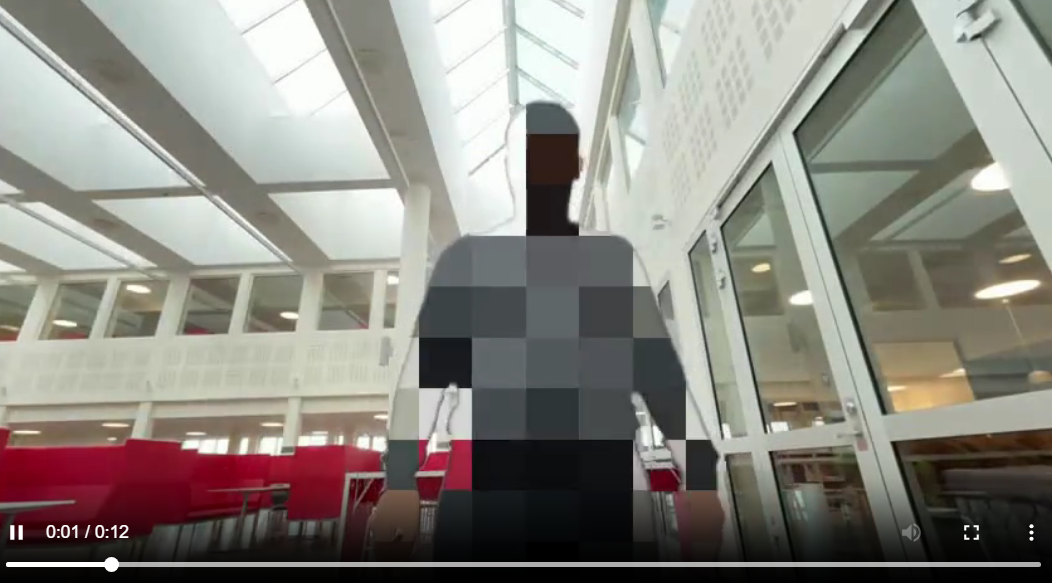
\includegraphics[width=\linewidth]{figures/images/chapter-11/segmentation pixelate video2.png}
\end{subfigure}
\hfill
\begin{subfigure}{0.48\textwidth}
\centering
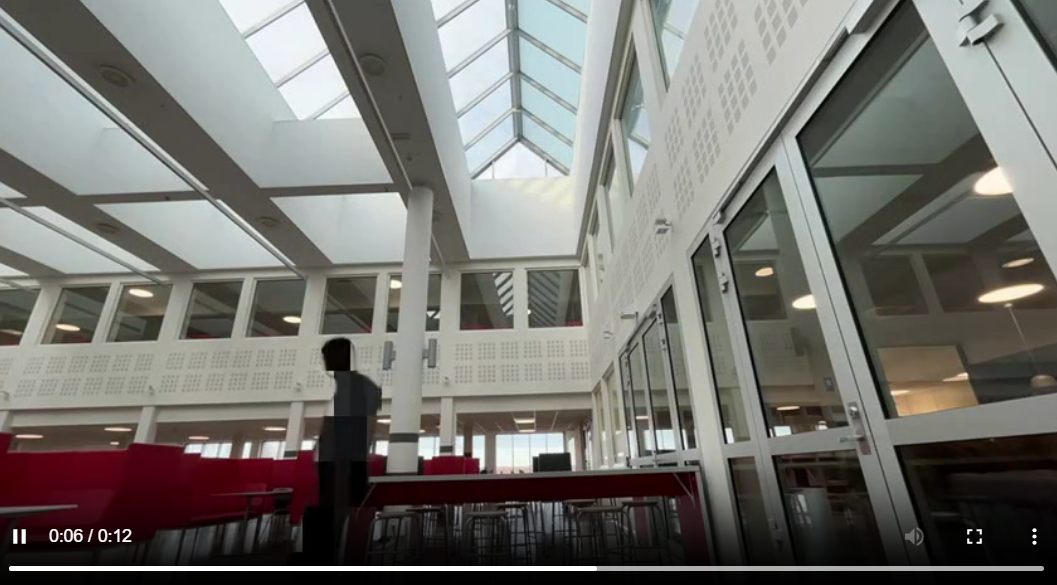
\includegraphics[width=\linewidth]{figures/images/chapter-11/segmentation pixelate video.png}
\end{subfigure}
\caption{Example of video redaction. The redaction stage uses the frame-wise manifest to apply \gls{segmentation} and pixelation to regions in the video. Video by authors.}
\label{fig:video_redaction_example}
\end{figure}

\methodheading{Automatic Kalman-Based Prediction Results}

Kalman-based prediction preserved accurate \gls{bounding box}es between detection frames, particularly when detector updates were performed frequently. Because full detection is only executed on selected frames, the most important evaluation cases were the non-detection frames, where object positions had to be estimated without new detector output.

\begin{table}[H]
\centering
\small
\setlength{\tabcolsep}{5pt}
\begin{tabular}{rcccc}
\toprule
\textbf{\texttt{detect\_every}} & \textbf{Boxes} & \textbf{Mean \acrshort{iou}} & \textbf{Mean coverage} & \textbf{$\geq$90\% coverage} \\
\midrule
2  & 819  & 0.963 & 0.982 & 98.7\% \\
5  & 1312 & 0.922 & 0.958 & 92.6\% \\
10 & 1475 & 0.851 & 0.920 & 80.1\% \\
\bottomrule
\end{tabular}

\caption{Kalman based prediction accuracy on non detection frames across the three evaluated videos. ``Boxes'' refers to human labeled boxes. Mean \acrshort{iou} measures bounding box alignment, while mean coverage measures how much of the human-labeled sensitive regions were covered by the predicted boxes.}
\label{tab:kalman_prediction_accuracy}
\end{table}

Frequent detector updates produced the strongest prediction results, as shown in Table~\ref{tab:kalman_prediction_accuracy}. With \texttt{detect\_every = 2}, the mean \acrshort{iou} reached 0.963 and the mean sensitive-region coverage reached 0.982, showing that the predicted boxes were both well aligned and able to cover nearly all labeled sensitive regions. With \texttt{detect\_every = 5}, the mean \acrshort{iou} decreased to 0.922, while mean coverage remained high at 0.958. This indicates that moderate detector skipping still preserved useful prediction accuracy for review and redaction.

A clearer degradation appeared with \texttt{detect\_every = 10}. In this configuration, mean \acrshort{iou} decreased to 0.851, and the share of boxes with at least 90\% coverage decreased to 80.1\%. Longer prediction intervals therefore increased localization drift, especially in difficult frames with fast motion, scale changes, or multiple nearby objects. Even so, the mean coverage remained 0.920, meaning that the predicted boxes still covered most sensitive regions despite less precise alignment. This distinction is important for \gls{SafeVision}, since anonymization depends not only on tight localization, but also on whether sensitive content is sufficiently covered.

\methodheading{Manual Tracking Results}

Manual tracking was evaluated separately from automatic Kalman-based prediction to assess whether a user-selected region could be propagated reliably across a video sequence. The evaluation used the \texttt{car\_video} sequence and compared tracked \gls{bounding box}es with manually labeled ground-truth boxes. This tested the manual tracking path described in Section~\ref{sec:video_imp}, where TrackerViT is used as the primary OpenCV tracker and \acrshort{csrt} is available as a fallback.

The qualitative examples in Figure~\ref{fig:manual_tracking_examples} illustrate both successful and unsuccessful tracking behaviour. The tracker followed the selected vehicle accurately during normal visibility and when the object appeared smaller in the frame, but also produced one \gls{false positive} after the vehicle had left the scene. The corresponding quantitative results are summarized in Table~\ref{tab:manual_tracking_results}.

\begin{figure}[H]
\centering

\begin{subfigure}{0.48\textwidth}
    \centering
    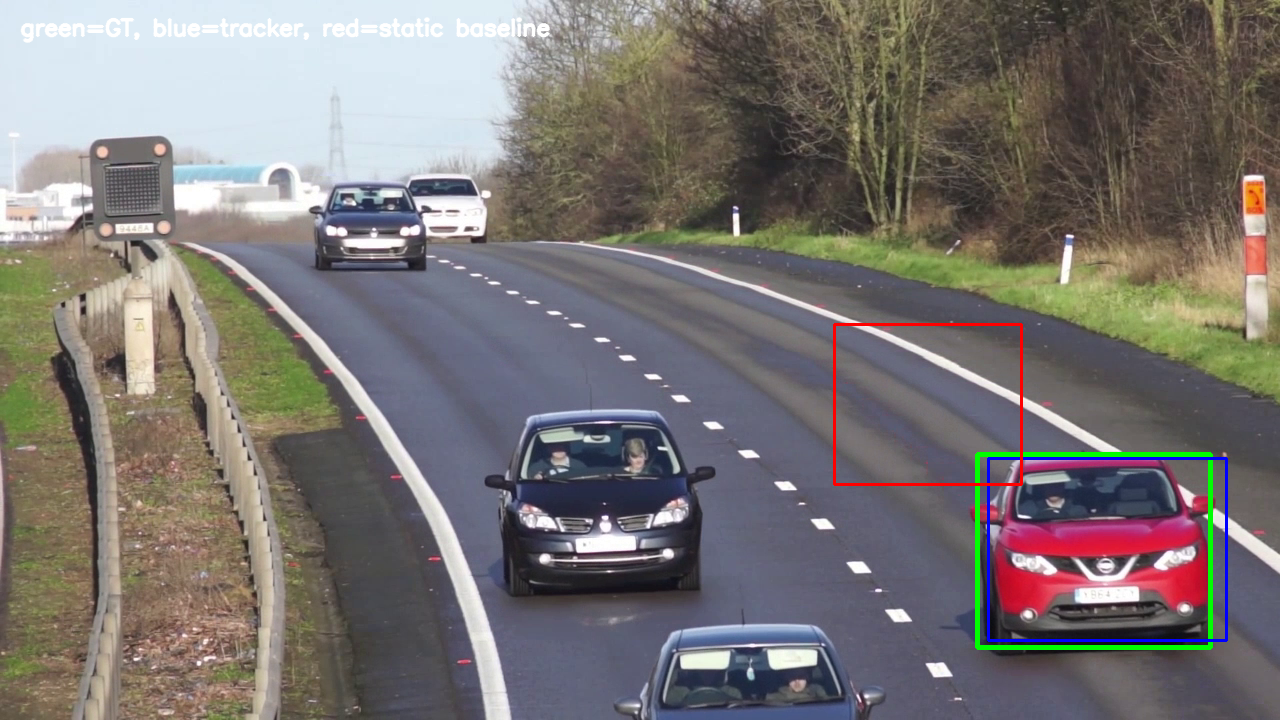
\includegraphics[width=\linewidth]{figures/images/chapter-11/car_track.png}
    \caption{Example of accurate manual tracking during normal object visibility.}
\end{subfigure}
\hfill
\begin{subfigure}{0.48\textwidth}
    \centering
    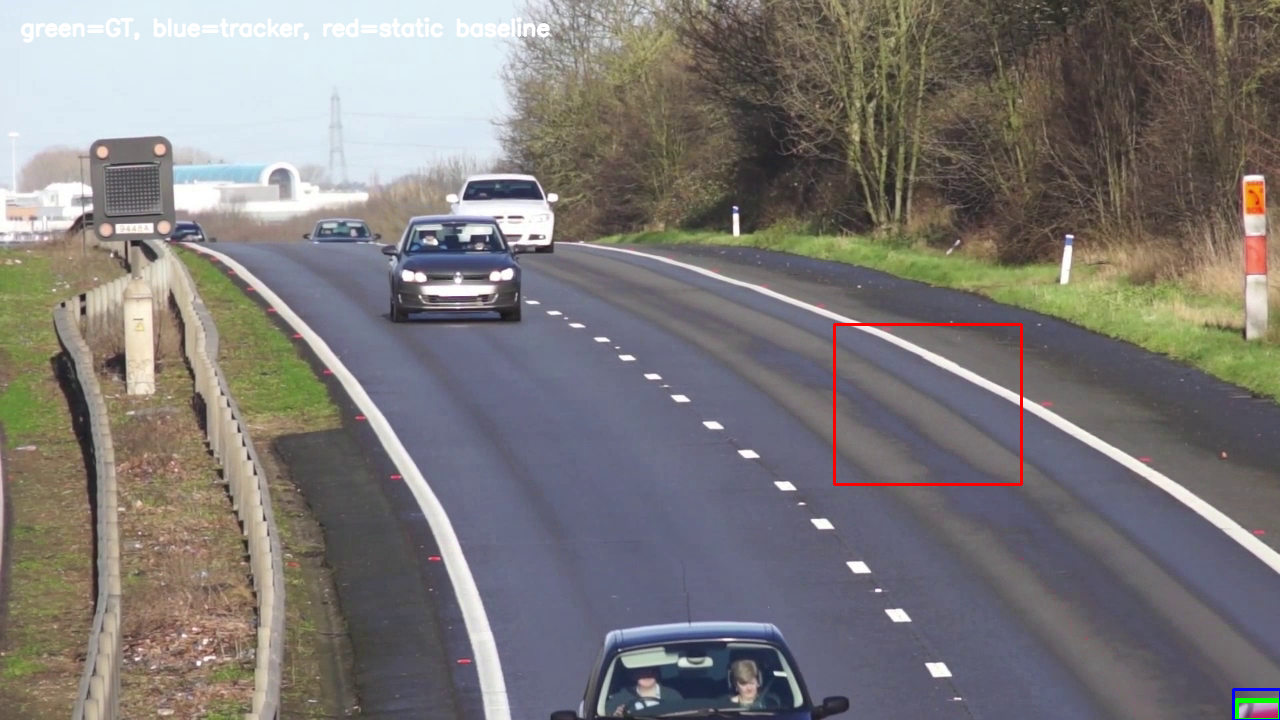
\includegraphics[width=\linewidth]{figures/images/chapter-11/false_car_track2.png}
    \caption{Example of accurate manual tracking during small object visibility.}
\end{subfigure}
\hfill
\begin{subfigure}{0.48\textwidth}
    \centering
    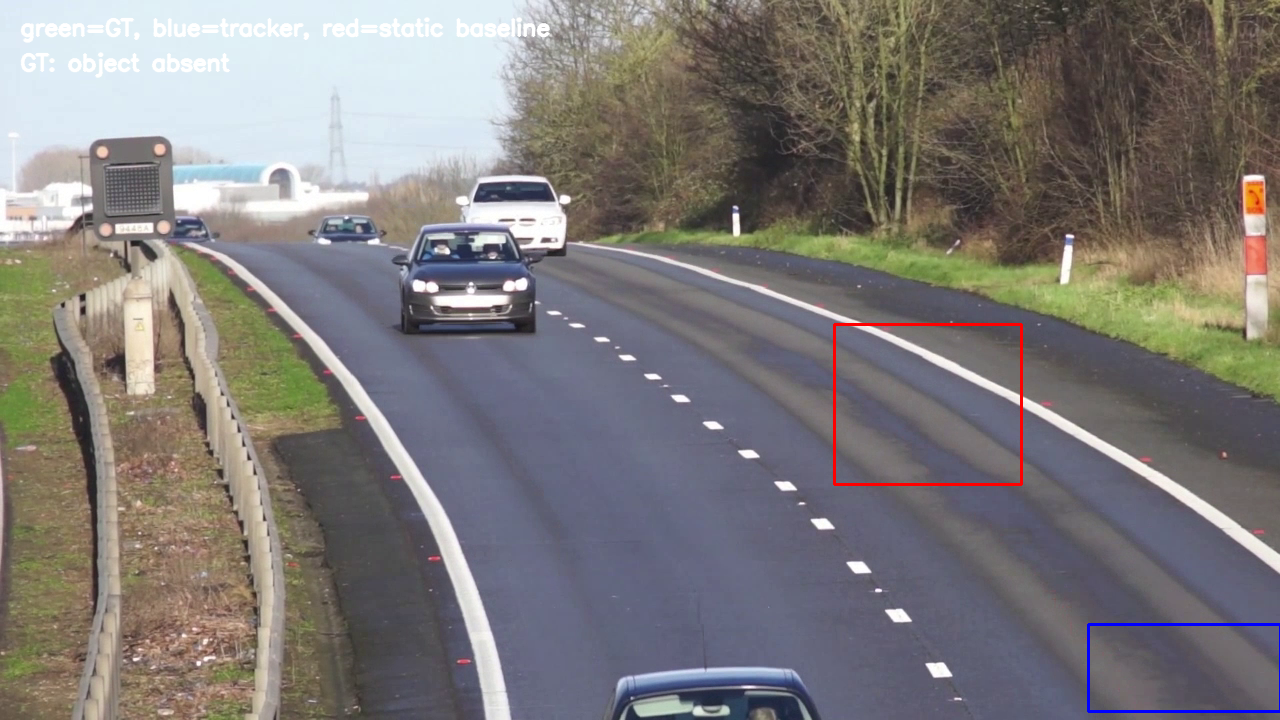
\includegraphics[width=\linewidth]{figures/images/chapter-11/false_car_track.png}
    \caption{Example of a \gls{false positive} after the object had left the scene.}
\end{subfigure}

\caption{Examples from the manual tracking evaluation. The red box shows the initial manually selected \gls{bounding box} used to start tracking, the green box shows the human-labeled ground truth, and the blue box shows the tracker output. Adapted from~\cite{pexels_highway_video}.}
\label{fig:manual_tracking_examples}
\end{figure}

\begin{table}[H]
\centering
\begin{tabular}{lc}
\toprule
\textbf{Metric} & \textbf{Result} \\
\midrule
Annotated frames & 25 \\
Visible annotated frames & 24 \\
Absent annotated frames & 1 \\
Mean \acrshort{iou} on visible frames & 0.8632 \\
Median \acrshort{iou} on visible frames & 0.8574 \\
Lowest \acrshort{iou} on visible frames & 0.6040 \\
Mean sensitive-region coverage & 0.9135 \\
Lowest sensitive-region coverage & 0.8188 \\
Missed visible frames & 0 \\
False positives on absent frames & 1 \\
Manual tracking runtime & 1.135 s \\
\bottomrule
\end{tabular}
\caption{Manual tracking results using human-labeled ground-truth boxes. Sensitive-region coverage measures how much of the human-labeled car region was covered by the tracked box.}
\label{tab:manual_tracking_results}
\end{table}

Across the visible frames, the manual tracker achieved a mean \acrshort{iou} of 0.8632 and a median \acrshort{iou} of 0.8574. The lowest visible-frame \acrshort{iou} was 0.6040, and the mean sensitive-region coverage was 0.9135, indicating that the tracked boxes generally remained well aligned with the annotated vehicle while also covering most of the sensitive region. No visible frames were missed, but one \gls{false positive} occurred after the vehicle had left the scene. These results show that manual tracking can support user-guided video redaction, but that user review remains important when an object leaves the frame, becomes occluded, or becomes difficult to distinguish from the background.

\methodheading{Processing Performance}

Processing performance was evaluated using different \texttt{detect\_every} values. This benchmark measured how detection frequency affected processing cost, while Table~\ref{tab:kalman_prediction_accuracy} shows the accuracy effect of the same configurations.

\begin{table}[H]
\centering
\begin{tabular}{rccc}
\toprule
\textbf{\texttt{detect\_every}} & \textbf{Detection calls} & \textbf{Processing time} & \textbf{Time reduction} \\
\midrule
1  & 261.00 & 231.71 s & -- \\
2  & 130.67 & 115.89 s & 50.0\% \\
5  & 52.33  & 46.61 s  & 79.9\% \\
10 & 26.33  & 23.57 s  & 89.8\% \\
\bottomrule
\end{tabular}
\caption{Average video processing time across the three tested videos for different detection intervals. Time reduction is calculated relative to running detection on every frame.}
\label{tab:video_processing_performance}
\end{table}

Reducing detection frequency substantially decreased processing time. Running full detection on every frame resulted in an average processing time of 231.71 seconds, while \texttt{detect\_every = 10} reduced the average processing time to 23.57 seconds. This corresponds to an approximate reduction of 89.8\%.

These results demonstrate why prediction is important for video processing in \gls{SafeVision}. Because the same detection models are reused for video frames, running all detectors on every frame is computationally expensive. By reducing the number of detector calls and using prediction between detection frames, the system can improve processing speed while still maintaining a frame-wise manifest for review and redaction. Among the tested configurations, \texttt{detect\_every = 5} provided the best balance between processing time and prediction accuracy, reducing processing time by 79.9\% while maintaining a mean \acrshort{iou} of 0.922 and mean ground-truth coverage of 0.958 on non-detection frames.